\documentclass{article}

% AlpaSim technical report (PAI track), team amanupg, final entry v7. Built on the organisers' template
% (alpasim_technical_report.tex, neurips_2026.sty in this folder); not a NeurIPS submission.
% DRAFT 2026-10-26. The v5-only version is amanupg_pai_report.tex. Items marked TODO wait on the final choice,
% the PAI warmup and the official v7 result.
\PassOptionsToPackage{numbers}{natbib}
\usepackage[preprint]{neurips_2026}
\makeatletter
\renewcommand{\@noticestring}{}
\makeatother

\usepackage[utf8]{inputenc}
\usepackage[T1]{fontenc}
\usepackage{hyperref}
\usepackage{booktabs}
\usepackage{xcolor}
\usepackage{amsmath}
\usepackage{tikz}
\usetikzlibrary{positioning,arrows.meta}

\newcommand{\todo}[1]{\textcolor{red}{[TODO: #1]}}

\title{Route Snap and Closed-Loop Fine-Tuning of a Vision-Language-Action Driver\\
\large AlpaSim E2E Closed Loop Challenge Technical Report (PAI track)}

\author{
  Team amanupg \\
  Aman Upganlawar, Columbia University \\
  \texttt{au2327@columbia.edu}
}

\begin{document}
\maketitle

\begin{abstract}
Our PAI-track entry drives with NVIDIA's Alpamayo~1.5 vision-language-action model behind a thin closed-loop
driver. Two additions address its closed-loop failures. \emph{Route snap} steers the plan onto the provided route
waypoints when the model ignores a lane change the route requires; it raised the official average scene score from
0.611 to 0.652. A \emph{closed-loop fine-tune} of the 2.3B-parameter flow-matching action expert, on frames rendered by
the simulator from the training split, including recovery states, is averaged with the released weights and paired
with the model's own route-text input. On 321 curated-validation scenes never used for any decision, with the
leaderboard's rendering, it raises the local mean scene score from 0.739 to 0.796 (+0.057, 90\% bootstrap interval
[+0.023,\,+0.093]) and cuts corridor exits from 37 to 22; a rule that starts the car when its plan keeps postponing
the start adds +0.004 with no scene worse. We also report a measurement finding that shaped every
decision: with the Harmonizer off, local closed-loop runs repeat bit for bit, so gains can be confirmed exactly on
held-out scenes.
\end{abstract}

\section{System}
The policy is the public Alpamayo~1.5 (10B)~\cite{alpamayo15}: a Qwen3-VL-8B backbone~\cite{qwen3vl} reads the four
front cameras (cross-left, front-wide, cross-right, front-tele; 4 frames at 0.1\,s, $576\times320$) and 16 ego poses,
and a 2.3B flow-matching action expert outputs 64 poses over 6.4\,s. Weights are int8 weight-only (torchao), the
token-embedding table stays on the CPU and all GPU work runs on one thread; the driver peaks at 14.6--15.2\,GB under
the 16\,GiB cap. It replans at 1\,Hz and serves the cached plan re-anchored to the current pose in between.

\begin{figure}[h]
\centering
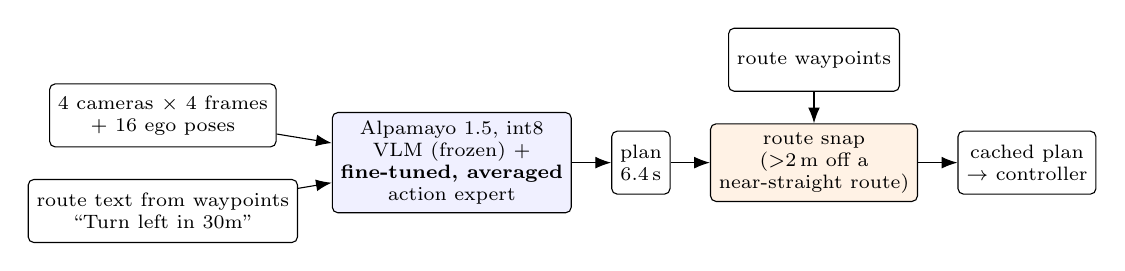
\begin{tikzpicture}[node distance=4mm and 5mm, font=\scriptsize,
  box/.style={draw, rounded corners=2pt, align=center, minimum height=8mm, inner sep=3pt},
  ar/.style={-{Latex[length=2mm]}}]
\node[box] (cam) {4 cameras $\times$ 4 frames\\+ 16 ego poses};
\node[box, below=of cam] (nav) {route text from waypoints\\``Turn left in 30m''};
\node[box, right=7mm of cam, yshift=-6mm, fill=blue!6] (a15) {Alpamayo 1.5, int8\\VLM (frozen) +\\\textbf{fine-tuned, averaged}\\action expert};
\node[box, right=of a15] (plan) {plan\\6.4\,s};
\node[box, right=of plan, fill=orange!10] (snap) {route snap\\($>$2\,m off a\\near-straight route)};
\node[box, above=of snap] (route) {route waypoints};
\node[box, right=of snap] (out) {cached plan\\$\rightarrow$ controller};
\draw[ar] (cam) -- (a15); \draw[ar] (nav) -- (a15); \draw[ar] (a15) -- (plan); \draw[ar] (plan) -- (snap);
\draw[ar] (route) -- (snap); \draw[ar] (snap) -- (out);
\end{tikzpicture}
\caption{Final system. Ours: route text from the waypoints, the fine-tuned and averaged expert, route snap, and the wait-then-go start fix (not drawn).}
\end{figure}

\textbf{Route text.} The route arrives as waypoints starting about 40\,m ahead. When a route segment within 100\,m
turns more than 30$^\circ$ from the car's heading, we pass Alpamayo's navigation input ``Turn left/right in
$X$m'', with $X$ where the turned road, extended back, meets the car's forward axis.

\textbf{Forced trajectory token.} In closed loop the model omitted \texttt{<traj\_future\_start>} in 30--42\% of
plans; we append it, as NVIDIA's teacher-forced training does.

\textbf{Route snap.} If the plan's mean distance to the route waypoints it reaches exceeds 2\,m (1\,m while a snap is
under way) and the route lies within 15$^\circ$ of the car's heading, the plan's geometry is replaced by a cubic Hermite
curve onto the route, re-timed so the model keeps control of speed. The angle guard stops corner cutting on turns.
On H100 it gave +0.071 [+0.011,\,+0.131] over the plain model on 120 scenes (official: 0.611 $\rightarrow$ 0.652).

\textbf{Wait-then-go start.} Stopped at a light, the model sometimes plans ``wait about 2\,s, then go'' at every replan,
so the start keeps receding and the non-reactive car behind ends the scene. When the car is stopped and three
consecutive plans cover under 1\,m in 2\,s but over 5\,m by 6.4\,s, we drop the waiting prefix so the car starts now.
On the 321 held-out scenes it changes 4 scenes, all for the better (e.g.\ 0.39 $\rightarrow$ 1.00), and no other.

\section{Closed-loop fine-tuning of the action expert}
Open loop, the released model is not slow on rendered on-route frames (predicted/recorded path length 1.005); its
closed-loop failures come from states the recording never visits. We fine-tune only the action expert and its
input/output projections (2.28B of 11.08B parameters; VLM frozen) with the flow-matching loss, on samples rendered by
AlpaSim from the NuRec curated \emph{training} split (no overlap with any validation scene we evaluate on), with the
exact input the driver sees:
(i) \emph{recording-following}: the ego is forced onto the recording; label = recorded 6.4\,s future (7.8k samples);
(ii) \emph{recovery} (DAgger-style~\cite{dagger}): our policy drives; the label starts at the ego's pose and blends onto
the recording over 3\,s with a cosine weight (1.4k samples; labels that jump back in 0.1\,s made the loss explode).
Two epochs, learning rate $3\cdot10^{-5}$, 2.0k steps of 8 samples, 5.5\,h on one 48\,GB GPU.

\textbf{bf16 updates.} With bf16 weights, \texttt{torch.optim.AdamW} at $10^{-5}$ silently drops updates (a 50-step
test moves 0.02 to 0.02002 instead of 0.0195). Stochastic rounding of the updated weight tracks the fp32 trajectory
without fp32 master weights, which would not fit beside the model.

\textbf{What mattered.} Recording-following data alone lowered held-out open-loop error by 21--24\% but was neutral
closed loop: the car tracked the recording and drove slower. Adding recovery samples gave +0.043 (two runs).
Averaging the fine-tuned and released expert weights 1:1 (WiSE-FT~\cite{wiseft}) restored speed (+0.049). Route text
did nothing with the released expert (+0.002) but added +0.036 with the averaged one, nearly halving corridor exits
(Table~\ref{tab:ladder}).

\textbf{A stronger teacher on the policy's own states.} We let the final policy drive 240 unused training scenes,
saved its 16 samples per plan (2{,}466 states, all six cameras, route text), and had Alpamayo~2-Super (34B) propose 8
plans per state with the same route text. Following RoaD~\cite{road}, the label is the candidate from either pool nearest
the recording over the first 2\,s (a recovery blend if none is within 3\,m): the policy's own sample in 62\% of states,
the teacher's in 26\%. Per sample the teacher is no closer to the recording than our policy (0.83 vs 0.82\,m), so its
value is diversity. A first run from our expert gave 20 more full passes and 14 fewer rear-end endings on the held-out
scenes but the same number of zero-score failures (+0.005 [$-$0.017,\,+0.027]); its training loss was flat, so we
retrained at the dose that worked for run C. At that dose, starting from our expert ($-$0.020 on the 120 screening
scenes), weighting each state by its scene's outcome (states before a zero-score ending take the teacher's or a
recovery target, $-$0.021), and RoaD alone ($-$0.058) all trained properly and none beat the final model.

\textbf{Seeds and soups.} Run C's exact recipe with other seeds was worse each time: one seed scored 0.051 below C
(raw experts, Harmonizer on), and two more, averaged and with route text like the final model, scored $-$0.034 and
$-$0.026 against it. C was a good draw. Averaging three seeds with the released weights was level with the final model
($+$0.003 [$-$0.033,\,+0.040]).

\section{Evaluation protocol}
\textbf{Determinism.} With the Harmonizer off, as in the leaderboard's initial runs, local closed-loop runs on one GPU
type repeat bit for bit (two runs of 120 scenes: every scene identical). The run-to-run variation we had seen
($\pm$0.05 per 40-scene batch) comes from the Harmonizer, a diffusion model, which the PAI final runs turn on.

\textbf{Held-out confirmation.} About 40 decisions were taken on 120 local scenes, so the final candidate was confirmed on
the 321 remaining curated-validation scenes (120 ``fresh'' plus a 201-scene lockbox kept untouched until the final
check), paired per scene with bootstrap 90\% intervals.

\textbf{Validity before verdicts.} A negative result only counts if the experiment was a real test: every fine-tune is
checked for a falling training loss and a weight change comparable to run C's before its closed-loop number is read,
and comparisons made with the Harmonizer on are reported as ``no detectable difference'' when inside its noise.
An audit by these rules caught one under-trained run and two earlier rejections made inside Harmonizer noise; all three
were retested.

\begin{table}[h]
\centering\small
\begin{tabular}{lcc}
\toprule
Screening scenes (120; L40S; Harmonizer on) & mean & vs v5 \\
\midrule
v5 (route snap, released expert; 2 runs) & 0.693 & -- \\
+ forced token & 0.707 & +0.013 \\
+ fine-tune C (recovery data; 2 runs) & 0.737 & +0.043 \\
+ C averaged 1:1 with released & 0.742 & +0.049 \\
\textbf{+ C averaged + route text (v7)} & \textbf{0.778} & \textbf{+0.084 [+0.027, +0.142]} \\
\bottomrule
\end{tabular}
\vspace{2mm}

\begin{tabular}{lccc}
\toprule
Held-out scenes, v5 $\rightarrow$ v7 & v5 & v7 & diff [90\%] \\
\midrule
321 scenes, Harmonizer off (deterministic) & 0.739 & 0.796 & \textbf{+0.057 [+0.023, +0.093]} \\
\quad corridor / offroad / at-fault (count) & 37 / 15 / 9 & 22 / 12 / 11 & \\
v7 $\rightarrow$ v7 + wait-then-go start (321) & 0.796 & 0.800 & +0.004 [+0.000, +0.009] \\
120 scenes, Harmonizer on (2 runs averaged) & 0.763 & 0.768 & +0.006 [$-$0.042, +0.053] \\
\bottomrule
\end{tabular}
\caption{Local closed-loop results. Official: v0.3 0.611 (PCS 2143); v5 0.652 (PCS 2184, 2219 after the
22~Oct re-scoring). \todo{official v7 result}}
\label{tab:ladder}
\end{table}

The gain holds on held-out scenes with the leaderboard's rendering; with the Harmonizer on, v7 is level with v5 on the
same scenes (no measurable gain or loss). Local gains have transferred to the leaderboard at about 0.6$\times$.

\textbf{What did not help} (all paired against the recipe of the time): reasoning text ($-$0.165); 5-sample medoid
($-$0.082); a 6-sample route chooser (+0.054 on one GPU type, +0.005 on H100); replanning at 2\,Hz ($-$0.045 with the chooser;
$-$0.049 on 40 scenes with v7); driving 15\% faster ($-$0.307); all six cameras ($-$0.023; rear-ends halved but own
failures rose); the organisers' time warp ($-$0.121); a waypoint memory to snap through turns (+0.003 to $-$0.026);
classifier-free guidance on route text, $w{=}2$ ($-$0.03); 40/60\% instead of 50\% averaging; more on-policy recovery
data ($-$0.029); RoaD-style own-sample labels~\cite{road} and Alpamayo~2-Super teacher labels from the released policy's
states (0.730/0.731 vs 0.742), and the same from the final policy's states (above; from the released expert $-$0.041);
NVIDIA's closest-lateral selection among 6 samples ($-$0.073);
a speed-aware snap bridge (+0.004); controller gains ($\le$+0.002, idx\_start\_penalty 5 or 15: $-$0.04 to $-$0.08);
route text in the fine-tuning prompts ($-$0.004); 20 flow-sampler steps instead of the 10 the expert was trained with
($-$0.051).

\section{Limitations and safety}
\textbf{Fragile lane and branch choices.} Zero-score corridor exits dominate the remaining loss (0.069 of 0.20 per
scene), and they flip in both directions under any change of the expert. On the 120 screening scenes (15 zero-score for
the final model), each of five properly trained fine-tunes fixed 0--4 of them but broke 4--9 others, while most
improved pace (up to six fewer rear-end endings and four more full passes); only the seed average did not add failures.
Average-case gains are cancelled by this churn: a policy whose lane choice is stable under small perturbations matters
more than one that is better on average. \textbf{Front-end collisions.} v7 adds four late frontal at-fault collisions on held-out scenes (it removes three of
v5's): it drives faster and sometimes closes on a slowing lead. \textbf{Signal compliance vs.\ progress.} Many
remaining low-progress scenes are stops at red or unclear signals where the recorded driver went (e.g.\ a right turn
on red); the non-reactive car behind then ends the scene. We did not override these stops. \textbf{Route snap trusts
the route.} Where the route disagrees with the recorded lane (some highway scenes) snapping hurts, and the snapped
path is not re-checked for obstacles; a deployed system would need a collision check.

\section{Resources and reproducibility}
\textbf{Weights:} Alpamayo~1.5~10B (OpenMDW-1.1 / Apache-2.0) and its Qwen3-VL backbone, as released, plus our
fine-tuned, averaged action expert (4.5\,GB, loaded before int8 quantization). \textbf{Training data:} frames rendered
by AlpaSim~\cite{alpasim} from the PAI-AV NuRec curated training split under its access terms; the recording labels
training samples only and is never used at inference. Alpamayo~2-Super was used only offline as a teacher in an
experiment that was not adopted; it is not in the image. \textbf{Compute:} one 48\,GB GPU per capture or training job
(A6000/L40S/RTX PRO 6000) on a university cluster. \textbf{Runtime:} v5 used 9{,}522 of 14{,}400\,s officially; v7
has the same model call. \todo{v7 warmup wave time and peak memory}

\begin{thebibliography}{9}
\bibitem{alpamayo15} NVIDIA. \newblock Alpamayo 1.5. \newblock \url{https://huggingface.co/nvidia/Alpamayo-1.5-10B}, 2026.
\bibitem{qwen3vl} Qwen Team. \newblock Qwen3-VL. \newblock \url{https://huggingface.co/Qwen/Qwen3-VL-8B-Instruct}, 2025.
\bibitem{alpasim} NVIDIA. \newblock AlpaSim. \newblock \url{https://github.com/NVlabs/alpasim}, 2026.
\bibitem{dagger} S. Ross, G. Gordon, D. Bagnell. \newblock A reduction of imitation learning and structured prediction
to no-regret online learning. \newblock AISTATS 2011.
\bibitem{wiseft} M. Wortsman et al. \newblock Robust fine-tuning of zero-shot models. \newblock CVPR 2022.
\bibitem{road} G. Garcia-Cobo et al. \newblock RoaD: Rollouts as demonstrations for closed-loop training of driving
policies. \newblock arXiv:2512.01993, 2025.
\end{thebibliography}

\end{document}
